\documentclass[
../../AuD-Zusammenfassung.tex,
]
{subfiles}

\externaldocument[ext:]{../../AuD-Zusammenfassung}
% Set Graphics Path, so pictures load correctly
\graphicspath{{../../}}

\begin{document}
\section{Graphen Algorithmen}
\subsection{Graphen}
Der abstrakter Datentyp der Graphen besteht im Grunde aus verschiedenen Knoten (vertices V), die Kanten (edges E) zu anderen Knoten haben. Sogesehen sind auch Bäume immer Graphen, wenn auch beschränkter.
\subsubsection{Gerichtete Graphen}
Gerichtete Graphen sind Graphen bei denen die edges E immer nur in eine Richtung sind. D.h., dass eine Kante von Knoten u nach Knoten v \textbf{nicht} gleichzusetzen ist wie eine Kante von Knoten v nach Knoten u. \\
In normaler Notation werden Kanten im Schema $(u,v)\in E$ angegeben, was eine Kante von Knoten u nach Knoten v darstellt.

\begin{minipage}[t]{\textwidth}
    \centering
    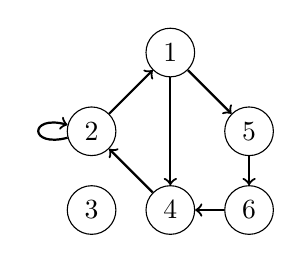
\begin{tikzpicture}[
        every node/.style={draw, minimum size=15pt, circle, text centered},
        ar/.style={->, thick},
        node distance = 22pt,
        invis/.style={draw=none},
    ]

    \node[](1) at (0,1) {1};
    \node[](4) at (0,-1) {4};
    \node[](2) at (-1,0) {2};
    \node[](5) at (1,0) {5};
    \node[](3) at (-1,-1) {3};
    \node[](6) at (1,-1) {6};

    \path[ar] 
    (1) edge (5) edge (4)
    (2) edge (1)

    (4) edge (2)
    (5) edge (6)
    (6) edge (4)
    ;
    \draw[ar, loop left] (2) to (2);
    \end{tikzpicture}
    \captionof*{figure}{Example}
    $V = \{1,2,3,4,5,6\}$\\
    $E = \{(1,4),(1,5),(2,1),(2,2),(4,2),(5,6),(6,4)\}$\\
    (3 hat keine Kanten weg oder zu sich, ist aber trotzdem Teil des Graphs)
\end{minipage}
\subsubsection{Ungerichtete Graphen}
Ungerichtete Graphen unterscheiden sich von gerichteten Graphen nur in der Hinsicht, dass die Kanten $(u,v)\in E$ und $(v,u) \in E$ gleichzusetzen sind.\\
\begin{minipage}[t]{\textwidth}
    \centering
    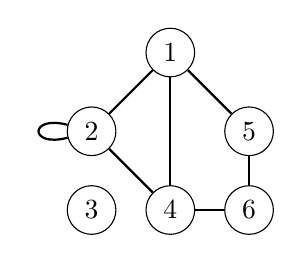
\begin{tikzpicture}[
        every node/.style={draw, minimum size=15pt, circle, text centered},
        ar/.style={-, thick},
        node distance = 22pt,
        invis/.style={draw=none},
    ]

    \node[](1) at (0,1) {1};
    \node[](4) at (0,-1) {4};
    \node[](2) at (-1,0) {2};
    \node[](5) at (1,0) {5};
    \node[](3) at (-1,-1) {3};
    \node[](6) at (1,-1) {6};

    \path[ar] 
    (1) edge (5) edge (4)
    (2) edge (1)

    (4) edge (2)
    (5) edge (6)
    (6) edge (4)
    ;
    \draw[ar, loop left] (2) to (2);
    \end{tikzpicture}
    \captionof*{figure}{Example}
    $V = \{1,2,3,4,5,6\}$\\
    $E = \{\{1,4\},\{1,5\},\{1,2\},\{2,2\}\{2,4\},\{4,6\},\{5,6\}\}$\\
    (Geschweifte Klammern stellen ungerichtete Kante dar)
\end{minipage}
\subsubsection{Pfade}
Ein Knoten $v$ ist von einem Knoten $u$ dann erreichbar, wenn es einen Pfad $(w_1,w_2,\ldots,w_k) \in V^k$ für den $(w_i,w_{i+1}) \in E$ für $i = 1,2,\ldots,k - 1$ und $w_1 = u$ und $w_k = v$ gibt.\\
(Ein Knoten ist immer von sich selbst erreichbar (leerer Pfad $k = 1$))\\
Dabei ist die Länge des Pfades mit $k - 1 =$ Anzahl der Kanten gegeben. $shortest(u,v) =$ Länge des kürzesten Pfades von $u$ nach $v$. 
\newpage
\subsubsection{Gewichtete Graphen}
Gewichtete Graphen haben zusätzlich bei den Kanten ein Gewicht. Dieses kann unterschiedliche Dinge, je nach Kontext bedeuten, bspw. könnte ein gewichteter Graph dazu genutzt werden Zugverbindungen darzustellen, wo die Knoten Haltestellen, die Kanten Zugverbindungen und die Gewichte die Entfernung darstellen. \\
Die Notation hierzu ist $w((u,v))$. Für ungerichtete gewichtete Graphen ist $w((u,v)) = w((v,u))$\\
\begin{minipage}[t]{\textwidth}
    \centering
    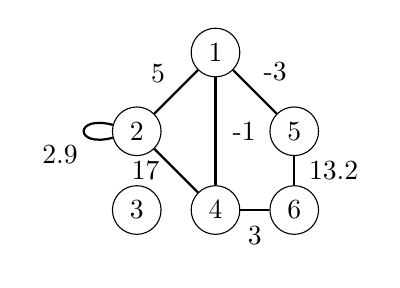
\begin{tikzpicture}[
        every node/.style={draw, minimum size=15pt, circle, text centered},
        ar/.style={-, thick},
        node distance = 22pt,
        invis/.style={draw=none},
    ]

    \node[](1) at (0,1) {1};
    \node[](4) at (0,-1) {4};
    \node[](2) at (-1,0) {2};
    \node[](5) at (1,0) {5};
    \node[](3) at (-1,-1) {3};
    \node[](6) at (1,-1) {6};

    \draw[ar] (1) to node[midway, above right, invis]{-3} (5);
    \draw[ar] (1) to node[midway, right, invis]{-1} (4);
    \draw[ar] (1) to node[midway, above left, invis]{5} (2);
    \draw[ar, loop left] (2) to node[midway, below left, invis]{2.9} (2);
    \draw[ar] (2) to node[midway, left, invis]{17} (4);
    \draw[ar] (4) to node[midway, below, invis]{3} (6);
    \draw[ar] (5) to node[midway, right, invis]{13.2} (6);


    \end{tikzpicture}
    \captionof*{figure}{Example}
\end{minipage}
\subsubsection{Zusammenhänge}
Ungerichtete Graphen gelten als \textbf{zusammenhängend}, wenn jeder Knoten von jedem anderen Knoten erreichbar ist. \\
\begin{minipage}[t]{0.5\textwidth}
    \centering
    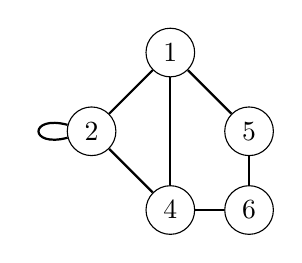
\begin{tikzpicture}[
        every node/.style={draw, minimum size=15pt, circle, text centered},
        ar/.style={-, thick},
        node distance = 22pt,
        invis/.style={draw=none},
    ]

    \node[](1) at (0,1) {1};
    \node[](4) at (0,-1) {4};
    \node[](2) at (-1,0) {2};
    \node[](5) at (1,0) {5};
    \node[](6) at (1,-1) {6};

    \path[ar] 
    (1) edge (5) edge (4)
    (2) edge (1)

    (4) edge (2)
    (5) edge (6)
    (6) edge (4)
    ;
    \draw[ar, loop left] (2) to (2);
    \end{tikzpicture}
    \captionof*{figure}{Zusammenhängend}
\end{minipage}
\begin{minipage}[t]{0.5\textwidth}
    \centering
    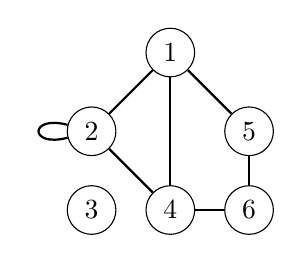
\begin{tikzpicture}[
        every node/.style={draw, minimum size=15pt, circle, text centered},
        ar/.style={-, thick},
        node distance = 22pt,
        invis/.style={draw=none},
    ]

    \node[](1) at (0,1) {1};
    \node[](4) at (0,-1) {4};
    \node[](2) at (-1,0) {2};
    \node[](5) at (1,0) {5};
    \node[](3) at (-1,-1) {3};
    \node[](6) at (1,-1) {6};

    \path[ar] 
    (1) edge (5) edge (4)
    (2) edge (1)

    (4) edge (2)
    (5) edge (6)
    (6) edge (4)
    ;
    \draw[ar, loop left] (2) to (2);
    \end{tikzpicture}
    \captionof*{figure}{Nicht zusammenhängend}
\end{minipage}
Ein gerichteter Graph gilt als \textbf{stark zusammenhängend}, wenn jeder Knoten von jedem anderen Knoten (beachte Kantenrichtung) erreichbar ist.\\
\begin{minipage}[t]{0.5\textwidth}
    \centering
    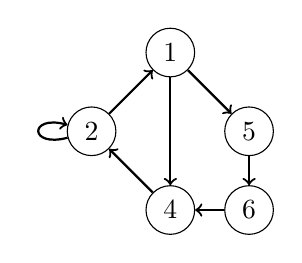
\begin{tikzpicture}[
        every node/.style={draw, minimum size=15pt, circle, text centered},
        ar/.style={->, thick},
        node distance = 22pt,
        invis/.style={draw=none},
    ]

    \node[](1) at (0,1) {1};
    \node[](4) at (0,-1) {4};
    \node[](2) at (-1,0) {2};
    \node[](5) at (1,0) {5};
    \node[](6) at (1,-1) {6};

    \path[ar] 
    (1) edge (5) edge (4)
    (2) edge (1)

    (4) edge (2)
    (5) edge (6)
    (6) edge (4)
    ;
    \draw[ar, loop left] (2) to (2);
    \end{tikzpicture}
    \captionof*{figure}{Zusammenhängend}
\end{minipage}
\begin{minipage}[t]{0.5\textwidth}
    \centering
    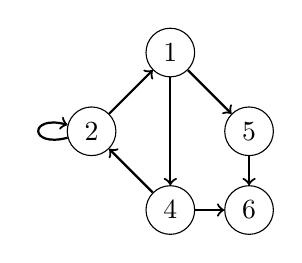
\begin{tikzpicture}[
        every node/.style={draw, minimum size=15pt, circle, text centered},
        ar/.style={->, thick},
        node distance = 22pt,
        invis/.style={draw=none},
    ]

    \node[](1) at (0,1) {1};
    \node[](4) at (0,-1) {4};
    \node[](2) at (-1,0) {2};
    \node[](5) at (1,0) {5};
    \node[](6) at (1,-1) {6};

    \path[ar] 
    (1) edge (5) edge (4)
    (2) edge (1)

    (4) edge (2) edge (6)
    (5) edge (6)
    ;
    \draw[ar, loop left] (2) to (2);
    \end{tikzpicture}
    \captionof*{figure}{Nicht zusammenhängend}
    Kein Pfad von 5 nach 1. (Richtung von (4,6) geändert)
\end{minipage}
\subsubsection{Subgraphen}
Ein Subgraph ist ein Graph, bei dem alle Kanten und Knoten auch in dem übergeordneten Graph liegen.\\
So gilt also $V_s \subseteq V $ und $E_s \subseteq E$.\\
\begin{minipage}[t]{0.5\textwidth}
    \centering
    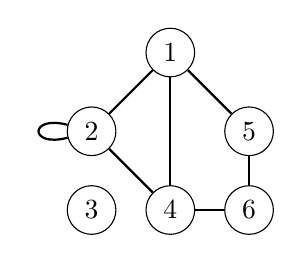
\begin{tikzpicture}[
        every node/.style={draw, minimum size=15pt, circle, text centered},
        ar/.style={-, thick},
        node distance = 22pt,
        invis/.style={draw=none},
    ]

    \node[](1) at (0,1) {1};
    \node[](4) at (0,-1) {4};
    \node[](2) at (-1,0) {2};
    \node[](5) at (1,0) {5};
    \node[](3) at (-1,-1) {3};
    \node[](6) at (1,-1) {6};

    \path[ar] 
    (1) edge (5) edge (4)
    (2) edge (1)

    (4) edge (2)
    (5) edge (6)
    (6) edge (4)
    ;
    \draw[ar, loop left] (2) to (2);
    \end{tikzpicture}
    \captionof*{figure}{Main Graph}
\end{minipage}
\begin{minipage}[t]{0.5\textwidth}
    \centering
    \begin{tikzpicture}[
        every node/.style={draw, minimum size=15pt, circle, text centered},
        ar/.style={-, thick},
        node distance = 22pt,
        invis/.style={draw=none},
    ]

    \node[](1) at (0,1) {1};
    \node[](4) at (0,-1) {4};
    \node[](2) at (-1,0) {2};
    \node[codegray!60](5) at (1,0) {5};
    \node[codegray!60](3) at (-1,-1) {3};
    \node[](6) at (1,-1) {6};

    \path[ar] 
    (1) edge (4)
    (2) edge (1)

    (6) edge (4)
    ;
    \draw[ar, loop left, codegray!60] (2) to (2);
    \draw[ar, codegray!60] (2) to (4);
    \draw[ar, codegray!60] (6) to (5);
    \draw[ar, codegray!60] (5) to (1);
    \end{tikzpicture}
    \captionof*{figure}{Subgraph}
\end{minipage}
\newpage
\subsubsection{Darstellungen}
\textbf{Adjazenzmatrix:}\\
Die Adjazenzliste stellt alle Kanten von einem Knoten zu anderen Knoten in jeder Zeile dar.\\[20pt]
\begin{minipage}[t]{0.5\textwidth}
    \centering
    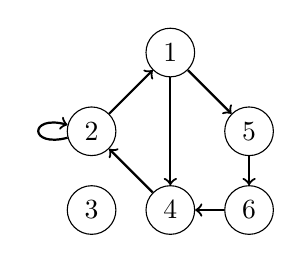
\begin{tikzpicture}[
        every node/.style={draw, minimum size=15pt, circle, text centered},
        ar/.style={->, thick},
        node distance = 22pt,
        invis/.style={draw=none},
    ]

    \node[](1) at (0,1) {1};
    \node[](4) at (0,-1) {4};
    \node[](3) at (-1,-1) {3};
    \node[](2) at (-1,0) {2};
    \node[](5) at (1,0) {5};
    \node[](6) at (1,-1) {6};

    \path[ar] 
    (1) edge (5) edge (4)
    (2) edge (1)

    (4) edge (2)
    (5) edge (6)
    (6) edge (4)
    ;
    \draw[ar, loop left] (2) to (2);
    \end{tikzpicture}
    \captionof*{figure}{Example}
\end{minipage}
\begin{minipage}[t]{0.5\textwidth}
    \centering
    \begin{tikzpicture}[
        array/.style={
            matrix of nodes, nodes={draw ,minimum size =15pt, fill=backcolour, anchor=south},
            row 1/.style={nodes={draw=none, fill=none, color=codegray}},
            row 2/.style={nodes={draw=none, fill=none, color=codegray}},
            column 1/.style={nodes={draw=none, fill=none, color=codegray}},
        },
    ]

    \matrix[array](m){
        to$\rightarrow$   &   &   &   &   &   &   \\
        from $\downarrow$ & 1 & 2 & 3 & 4 & 5 & 6 \\
                        1 & 0 & 0 & 0 & 1 & 1 & 0 \\
                        2 & 1 & 1 & 0 & 0 & 0 & 0 \\
                        3 & 0 & 0 & 0 & 0 & 0 & 0 \\
                        4 & 0 & 1 & 0 & 0 & 0 & 0 \\
                        5 & 0 & 0 & 0 & 0 & 0 & 1 \\
                        6 & 0 & 0 & 0 & 1 & 0 & 0 \\
    };
    \end{tikzpicture}
\end{minipage}\\[20pt]
Für ungerichtete Graphen ist die Adjazenzmatrix spiegelsymmetrisch zur Hauptdiagonalen.\\
Die Adjazenzmatrix hat die Eigenschaft, dass der Eintrag $a_{i,j}^{(m)}$ ($i$-te Zeile, $j$-te Spalte der $m$-ten ($A^m$) Potenz der Matrix $A$) die Anzahl der Wege von Knoten $i$ zum Knoten $j$ mit genau $m$ Kanten besitzt.

\textbf{Adjazenzliste:}\\
Die Adjazenliste stellt die Kanten von einem Knoten zu anderen Knoten als Array mit verketteten Listen dar.\\[20pt]
\begin{minipage}[t]{0.5\textwidth}
    \centering
    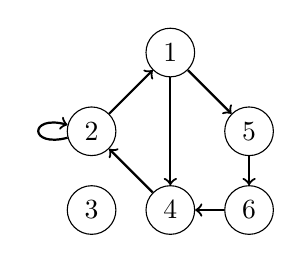
\begin{tikzpicture}[
        every node/.style={draw, minimum size=15pt, circle, text centered},
        ar/.style={->, thick},
        node distance = 22pt,
        invis/.style={draw=none},
    ]

    \node[](1) at (0,1) {1};
    \node[](4) at (0,-1) {4};
    \node[](3) at (-1,-1) {3};
    \node[](2) at (-1,0) {2};
    \node[](5) at (1,0) {5};
    \node[](6) at (1,-1) {6};

    \path[ar] 
    (1) edge (5) edge (4)
    (2) edge (1)

    (4) edge (2)
    (5) edge (6)
    (6) edge (4)
    ;
    \draw[ar, loop left] (2) to (2);
    \end{tikzpicture}
    \captionof*{figure}{Example}
\end{minipage}
\begin{minipage}[t]{0.5\textwidth}
    \centering
    \begin{tikzpicture}[
        invis/.style={draw=none, minimum size = 15pt, fill=none, color=codegray, anchor=south},
        table/.style={minimum width=25pt, minimum height=15pt, draw, rectangle, anchor=south},
        linked/.style={minimum width = 20pt, minimum height = 12.5pt, draw, rectangle, rounded corners},
        ar/.style={<->, thick},
        node distance = 20pt,
    ]

    \node[invis](1i){1};
    \node[invis, below = 0 of 1i](2i){2};
    \node[invis, below = 0 of 2i](3i){3};
    \node[invis, below = 0 of 3i](4i){4};
    \node[invis, below = 0 of 4i](5i){5};
    \node[invis, below = 0 of 5i](6i){6};


    \node[table, right = 0 of 1i](1-1){4};
    \node[table, right = of 1-1](1-2){5};

    \node[table, below = 0 of 1-1](2-1){1};
    \node[table, right = of 2-1](2-2){2};

    \node[table, below = 0 of 2-1](3-1){};

    \node[table, below = 0 of 3-1](4-1){2};

    \node[table, below = 0 of 4-1](5-1){6};

    \node[table, below = 0 of 5-1](6-1){4};

    \draw[ar] (1-1) to (1-2);
    \draw[ar] (2-1) to (2-2);

    \end{tikzpicture}
\end{minipage}

\newpage
\subsection{Breadth-First Search (BFS)}
Der Breadth-First Search Algorithmus funktioniert nach dem Prinzip, dass von dem Startpunkt aus erst alle direkten Nachbarn besucht werden. Anschließend werden alle Nachbarn der direkten Nachbarn besucht und so weiter.\\
Allgemein basiert dieser Algorithmus also eher auf der Queue Mechanik, er fügt zuerst alle Werte hinzu und bearbeitet dann den zuerst hinzugefügten Wert. \\
\begin{algorithm}[H]
    \SetKwFunction{BFS}{breadthFirstSearch}
    \tcp{G: graph with (V,E), s: start}
    \Fn{\BFS{G,s}}{
        \tcp{for all nodes except s:}
        \ForEach{u in V-\{s\}}{
            u.color = WHITE; 
            u.dist = $+\infty$; 
            u.pred = \KwNil; \tcp{Initializes all nodes to appropriate values}

        }
        s.color = GRAY; 
        s.dist = 0; 
        s.pred = \KwNil; \tcp{Initializes s at the first node}
        Q = new Queue(); \tcp{Initializes queue for saving order}
        Q.enqueue(s); \tcp{add s as first node to queue}
        \tcp{While there is an unfinished node with a path from s:}
        \While{!isEmpty(Q)}{
            u = Q.dequeue()\;
            \tcp{For all nodes adjacent to u:}
            \ForEach{ v in Adj(u)}{
                \tcp{If v has not been visited yet:}
                \If{v.color == WHITE}{
                    v.color = GRAY; \tcp{Mark node as visited}
                    v.dist = u.dist + 1; \tcp{set distance}
                    v.pred = u; \tcp{set predecessor}
                    Q.enqueue(v); \tcp{Add node to queue}
                }
            }
            u.color = BLACK; \tcp{Mark current node as finished}
        }
    }
\end{algorithm}
In diesem Code wird der Status der Knoten über Farben angegeben. \texttt{WHITE} bedeutet noch nicht besucht, \texttt{GRAY} bedeutet besucht, \texttt{BLACK} bedeutet beendet.\\
\begin{minipage}[t]{0.33\textwidth}
    \centering
    \begin{tikzpicture}[
        every node/.style={draw, minimum size=15pt, circle, text centered},
        ar/.style={->, thick},
        node distance = 22pt,
        invis/.style={draw=none},
        queued/.style={fill=codegray!50},
        finished/.style={fill=codegray},
    ]

    \node[queued](1) at (0,1) {1};
    \node[](4) at (0,-1) {4};
    \node[](2) at (-1,0) {2};
    \node[](5) at (1,0) {5};
    \node[](3) at (-1,-1) {3};
    \node[](6) at (1,-1) {6};

    \node[invis, above =-15pt of 1] {\small(0/NIL)}; 

    \path[ar] 
    (1) edge (5) edge (4)
    (2) edge (1)

    (4) edge (2) edge (5)
    (5) edge (6)
    (6) edge (4)
    ;
    \draw[ar, loop left] (2) to (2);
    \end{tikzpicture}\\
    Q = (1)
\end{minipage}
\begin{minipage}[t]{0.33\textwidth}
    \centering
    \begin{tikzpicture}[
        every node/.style={draw, minimum size=15pt, circle, text centered},
        ar/.style={->, thick},
        node distance = 22pt,
        invis/.style={draw=none},
        queued/.style={fill=codegray!50},
        finished/.style={fill=codegray},
    ]

    \node[finished](1) at (0,1) {1};
    \node[queued](4) at (0,-1) {4};
    \node[](2) at (-1,0) {2};
    \node[queued](5) at (1,0) {5};
    \node[](3) at (-1,-1) {3};
    \node[](6) at (1,-1) {6};

    \node[invis, below =-10pt of 4] {\small(1/1)}; 
    \node[invis, above =-10pt of 5] {\small(1/1)}; 

    \path[ar] 
    (1) edge (5) edge (4)
    (2) edge (1)

    (4) edge (2) edge (5)
    (5) edge (6)
    (6) edge (4)
    ;
    \draw[ar, loop left] (2) to (2);
    \end{tikzpicture}\\
    Q = (4,5)
\end{minipage}
\begin{minipage}[t]{0.33\textwidth}
    \centering
    \begin{tikzpicture}[
        every node/.style={draw, minimum size=15pt, circle, text centered},
        ar/.style={->, thick},
        node distance = 22pt,
        invis/.style={draw=none},
        queued/.style={fill=codegray!50},
        finished/.style={fill=codegray},
    ]

    \node[finished](1) at (0,1) {1};
    \node[finished](4) at (0,-1) {4};
    \node[queued](2) at (-1,0) {2};
    \node[queued](5) at (1,0) {5};
    \node[](3) at (-1,-1) {3};
    \node[](6) at (1,-1) {6};

    \node[invis, above =-10pt of 2] {\small(2/4)}; 
    \node[invis, above =-10pt of 5] {\small(1/1)}; 

    \path[ar] 
    (1) edge (5) edge (4)
    (2) edge (1)

    (4) edge (2) edge (5)
    (5) edge (6)
    (6) edge (4)
    ;
    \draw[ar, loop left] (2) to (2);
    \end{tikzpicture}\\
    Q = (5,2)
\end{minipage}\\[20pt]
\begin{minipage}[t]{0.33\textwidth}
    \centering
    \begin{tikzpicture}[
        every node/.style={draw, minimum size=15pt, circle, text centered},
        ar/.style={->, thick},
        node distance = 22pt,
        invis/.style={draw=none},
        queued/.style={fill=codegray!50},
        finished/.style={fill=codegray},
    ]

    \node[finished](1) at (0,1) {1};
    \node[finished](4) at (0,-1) {4};
    \node[queued](2) at (-1,0) {2};
    \node[finished](5) at (1,0) {5};
    \node[](3) at (-1,-1) {3};
    \node[queued](6) at (1,-1) {6};

    \node[invis, above =-10pt of 2] {\small(2/4)};
    \node[invis, below =-10pt of 6] {\small(2/5)}; 

    \path[ar] 
    (1) edge (5) edge (4)
    (2) edge (1)

    (4) edge (2) edge (5)
    (5) edge (6)
    (6) edge (4)
    ;
    \draw[ar, loop left] (2) to (2);
    \end{tikzpicture}\\
    Q = (2,6)
\end{minipage}
\begin{minipage}[t]{0.33\textwidth}
    \centering
    \begin{tikzpicture}[
        every node/.style={draw, minimum size=15pt, circle, text centered},
        ar/.style={->, thick},
        node distance = 22pt,
        invis/.style={draw=none},
        queued/.style={fill=codegray!50},
        finished/.style={fill=codegray},
    ]

    \node[finished](1) at (0,1) {1};
    \node[finished](4) at (0,-1) {4};
    \node[finished](2) at (-1,0) {2};
    \node[finished](5) at (1,0) {5};
    \node[](3) at (-1,-1) {3};
    \node[queued](6) at (1,-1) {6};

    \node[invis, below =-10pt of 6] {\small(2/5)}; 

    \path[ar] 
    (1) edge (5) edge (4)
    (2) edge (1)

    (4) edge (2) edge (5)
    (5) edge (6)
    (6) edge (4)
    ;
    \draw[ar, loop left] (2) to (2);
    \end{tikzpicture}\\
    Q = (6)
\end{minipage}
\begin{minipage}[t]{0.33\textwidth}
    \centering
    \begin{tikzpicture}[
        every node/.style={draw, minimum size=15pt, circle, text centered},
        ar/.style={->, thick},
        node distance = 22pt,
        invis/.style={draw=none},
        queued/.style={fill=codegray!50},
        finished/.style={fill=codegray},
    ]

    \node[finished](1) at (0,1) {1};
    \node[finished](4) at (0,-1) {4};
    \node[finished](2) at (-1,0) {2};
    \node[finished](5) at (1,0) {5};
    \node[](3) at (-1,-1) {3};
    \node[finished](6) at (1,-1) {6};

    \node[invis,rectangle, below =0pt of 3] {\small($+\infty$/NIL)}; 

    \path[ar] 
    (1) edge (5) edge (4)
    (2) edge (1)

    (4) edge (2) edge (5)
    (5) edge (6)
    (6) edge (4)
    ;
    \draw[ar, loop left] (2) to (2);
    \end{tikzpicture}\\
    Q = ()
\end{minipage}\\[20pt]

Der erste Wert in den Klammern ist der Schritt, an dem der Knoten entdeckt wurde. Der zweite Wert ist der Vorgängerknoten.
\newpage
Nach dem Ausführen von BFS kann man durch die jetzt gegebenen Vorgängern einen Subgraphen ableiten.\\
\begin{minipage}[t]{0.5\textwidth}
    \centering
    \begin{tikzpicture}[
        every node/.style={draw, minimum size=15pt, circle, text centered},
        ar/.style={->, thick},
        node distance = 22pt,
        invis/.style={draw=none, rectangle},
        queued/.style={fill=codegray!50},
        finished/.style={fill=codegray},
    ]

    \node[finished](1) at (0,1) {1};
    \node[finished](4) at (0,-1) {4};
    \node[finished](2) at (-1,0) {2};
    \node[finished](5) at (1,0) {5};
    \node[](3) at (-1,-1) {3};
    \node[finished](6) at (1,-1) {6};

    \node[invis, below =9.5pt of 3.west] {\small($+\infty$/NIL)}; 
    \node[invis, above =0 of 1] {\small(0/NIL)};
    \node[invis, above =0 of 5] {\small(1/1)};
    \node[invis, below =0 of 4] {\small(1/1)};
    \node[invis, below =0 of 6] {\small(2/5)};
    \node[invis, above =0 of 2] {\small(2/4)};

    \path[ar] 
    (1) edge (5) edge (4)
    (2) edge (1)

    (4) edge (2) edge (5)
    (5) edge (6)
    (6) edge (4)
    ;
    \draw[ar, loop left] (2) to (2);
    \end{tikzpicture}
    \captionof*{figure}{Graph nach BFS}
\end{minipage}
\begin{minipage}[t]{0.5\textwidth}
    \centering
    \begin{tikzpicture}[
        every node/.style={draw, minimum size=15pt, circle, text centered},
        ar/.style={->, thick},
        node distance = 20pt,
    ]
    \node[](1){1};
    \node[below left =of 1](4){4};
    \node[below right =of 1](5){5};
    \node[below =15pt of 4](2){2};
    \node[below =15pt of 5](6){6};

    \path[ar]
    (1) edge (4) edge (5)
    (4) edge (2)
    (5) edge (6)
    ;
    \end{tikzpicture}\\
    \captionof*{figure}{Abgeleiteter Subgraph}
\end{minipage}\\[20pt]
Der Subgraph ist durch $V_{pred}^s = \{v \in V | v.pred \not= $NIL$\} \cup \{s\}$ und $E_{pred}^s = \{(v.pred, v) | v \in V_{pred}^s - \{s\}\}$ gegeben. D.h. bedeutet, dass der Subgraph alle von $s$ erreichbaren Knoten enthält und für jeden Knoten im Subgraph genau ein Pfad von $s$, der auch automatisch der kürzeste Pfad von $s$ zu $v$ ist, existiert.

Um alle Knoten auf dem kürzesten Pfad zwischen zwei Knoten auszugeben kann der folgende Algorithmus verwendet werden.\\
\begin{algorithm}
    \SetKwFunction{psp}{printShortestPath}
    \tcp{G: Graph mit (V,E), s: Startknoten, v: Zielknoten}
    \Fn{\psp{G, s, v}}{
        \tcp{if end == start:}
        \If{v == s}{
            \KwPrint{s}\;
        } \tcp{if end nodes predecessor is NIL (no path):}
        \ElseIf {v.pred == \KwNil}{
            \KwPrint{"no path from s to v"}\;
        } \Else {
            \psp{G, s, v.pred}; \tcp{Recursion (backwards from end to start)}
            \KwPrint{v}\;
        }
    }
\end{algorithm}
\includepdf[pages={20,29}, pagecommand={},nup=1x2, frame=true, scale=0.9]{./VL Folien/06GraphAlgorithms.pdf}
\subsection{Depth-First Search (DFS)}
Das Prinzip des Depth-First Search Algorithmus ist, dass im Gegensatz zu BFS nicht erst alle Nachbarn eines Knotens besucht werden, sondern immer erst ein Pfad zuende gebracht wird, bevor ein anderer besucht wird. Der Algorithmus geht also solange einen Pfad ab, bis er an einem Knoten keine neuen Knoten mehr findet, wodurch er dann einen Knoten zurück geht und von diesem den nächsten Pfad abgeht. Dies macht er solange, bis er alle Pfade abgelaufen ist.\\ Allgemein kann man als Unterschied zu BFS sagen, dass dieser Algorithmus mehr der Stack Datenstruktur ähnelt, da sie zuerst die Knoten merkt und dann den zuletzt hinzugefügten Knoten verarbeitet.\\
\begin{algorithm}[H]
    \SetKwFunction{DFS}{depthFirstSearch}
    \SetKwFunction{visit}{visit}
    \tcp{G: graph with (V,E)}
    \Fn{\DFS{G}}{
        \tcp{for all nodes in the graph:}
        \ForEach{u in V}{
            u.color = WHITE; 
            u.pred = \KwNil; \tcp{Initializes all nodes to appropriate values}
        }
        time = 0; \tcp{Initializes time to 0}
        \tcp{for all nodes in the graph:}
        \ForEach{u in V}{
            \tcp{if node not visited:}
            \If{u.color == WHITE}{
                \visit{G,u}\;
            }
        }
    }

    \Fn{\visit{G,u}}{
        u.color = GRAY;
        u.disc = ++time \tcp{Mark node as visited and set discorvery time}
        \tcp{for all nodes adjacent to u:}
        \ForEach{v in u.adj}{
            \tcp{if node not visited:}
            \If{v.color == WHITE}{
                v.pred = u; \tcp{set predecessor}
                \visit{G,v}\;
            }
        }
        u.color = BLACK; 
        u.finish = ++time; \tcp{Mark node as finshed and set finish time}
    }
\end{algorithm}
Der Algorithmus hat im Gegensatz zu BFS keinen angegebenen Startknoten, sondern geht die Knoten nach natural Order an. 
\newpage
\begin{minipage}[t]{0.33\textwidth}
    \centering
    \begin{tikzpicture}[
        every node/.style={draw, minimum size=15pt, circle, text centered},
        ar/.style={->, thick},
        node distance = 22pt,
        invis/.style={rectangle,draw=none},
        queued/.style={fill=codegray!50},
        finished/.style={fill=codegray},
    ]

    \node[queued](1) at (0,1) {1};
    \node[](4) at (0,-1) {4};
    \node[](2) at (-1,0) {2};
    \node[](5) at (1,0) {5};
    \node[](3) at (-1,-1) {3};
    \node[](6) at (1,-1) {6};

    \node[invis, above =0 of 1] {\small(1/-/NIL)};
    \node[invis, above =9.5pt of 2.west] {\small(-/-/NIL)};
    \node[invis, below =9.5pt of 3.west] {\small(-/-/NIL)};
    \node[invis, below =0 of 4] {\small(-/-/NIL)};
    \node[invis, above =9.5pt of 5.east] {\small(-/-/NIL)};
    \node[invis, below =9.5pt of 6.east] {\small(-/-/NIL)};

    \path[ar] 
    (1) edge (5) edge (4)
    (2) edge (1)

    (4) edge (2) edge (5)
    (5) edge (6)
    (6) edge (2)
    ;
    \draw[ar, loop left] (2) to (2);
    \end{tikzpicture}
\end{minipage}
\begin{minipage}[t]{0.33\textwidth}
    \centering
    \begin{tikzpicture}[
        every node/.style={draw, minimum size=15pt, circle, text centered},
        ar/.style={->, thick},
        node distance = 22pt,
        invis/.style={rectangle,draw=none},
        queued/.style={fill=codegray!50},
        finished/.style={fill=codegray},
    ]

    \node[queued](1) at (0,1) {1};
    \node[queued](4) at (0,-1) {4};
    \node[](2) at (-1,0) {2};
    \node[](5) at (1,0) {5};
    \node[](3) at (-1,-1) {3};
    \node[](6) at (1,-1) {6};

    \node[invis, above =0 of 1] {\small(1/-/NIL)};
    \node[invis, above =9.5pt of 2.west] {\small(-/-/NIL)};
    \node[invis, below =9.5pt of 3.west] {\small(-/-/NIL)};
    \node[invis, below =0 of 4] {\small(2/-/1)};
    \node[invis, above =9.5pt of 5.east] {\small(-/-/NIL)};
    \node[invis, below =9.5pt of 6.east] {\small(-/-/NIL)};

    \path[ar] 
    (1) edge (5) edge (4)
    (2) edge (1)

    (4) edge (2) edge (5)
    (5) edge (6)
    (6) edge (2)
    ;
    \draw[ar, loop left] (2) to (2);
    \end{tikzpicture}
\end{minipage}
\begin{minipage}[t]{0.33\textwidth}
    \centering
    \begin{tikzpicture}[
        every node/.style={draw, minimum size=15pt, circle, text centered},
        ar/.style={->, thick},
        node distance = 22pt,
        invis/.style={rectangle,draw=none},
        queued/.style={fill=codegray!50},
        finished/.style={fill=codegray},
    ]

    \node[queued](1) at (0,1) {1};
    \node[queued](4) at (0,-1) {4};
    \node[queued](2) at (-1,0) {2};
    \node[](5) at (1,0) {5};
    \node[](3) at (-1,-1) {3};
    \node[](6) at (1,-1) {6};

    \node[invis, above =0 of 1] {\small(1/-/NIL)};
    \node[invis, above =9.5pt of 2.west] {\small(3/-/4)};
    \node[invis, below =9.5pt of 3.west] {\small(-/-/NIL)};
    \node[invis, below =0 of 4] {\small(2/-/1)};
    \node[invis, above =9.5pt of 5.east] {\small(-/-/NIL)};
    \node[invis, below =9.5pt of 6.east] {\small(-/-/NIL)};

    \path[ar] 
    (1) edge (5) edge (4)
    (2) edge (1)

    (4) edge (2) edge (5)
    (5) edge (6)
    (6) edge (2)
    ;
    \draw[ar, loop left] (2) to (2);
    \end{tikzpicture}
\end{minipage}\\[20pt]
\begin{minipage}[t]{0.33\textwidth}
    \centering
    \begin{tikzpicture}[
        every node/.style={draw, minimum size=15pt, circle, text centered},
        ar/.style={->, thick},
        node distance = 22pt,
        invis/.style={rectangle,draw=none},
        queued/.style={fill=codegray!50},
        finished/.style={fill=codegray},
    ]

    \node[queued](1) at (0,1) {1};
    \node[queued](4) at (0,-1) {4};
    \node[finished](2) at (-1,0) {2};
    \node[](5) at (1,0) {5};
    \node[](3) at (-1,-1) {3};
    \node[](6) at (1,-1) {6};

    \node[invis, above =0 of 1] {\small(1/-/NIL)};
    \node[invis, above =9.5pt of 2.west] {\small(3/4/4)};
    \node[invis, below =9.5pt of 3.west] {\small(-/-/NIL)};
    \node[invis, below =0 of 4] {\small(2/-/1)};
    \node[invis, above =9.5pt of 5.east] {\small(-/-/NIL)};
    \node[invis, below =9.5pt of 6.east] {\small(-/-/NIL)};

    \path[ar] 
    (1) edge (5) edge (4)
    (2) edge (1)

    (4) edge (2) edge (5)
    (5) edge (6)
    (6) edge (2)
    ;
    \draw[ar, loop left] (2) to (2);
    \end{tikzpicture}
\end{minipage}
\begin{minipage}[t]{0.33\textwidth}
    \centering
    \begin{tikzpicture}[
        every node/.style={draw, minimum size=15pt, circle, text centered},
        ar/.style={->, thick},
        node distance = 22pt,
        invis/.style={rectangle,draw=none},
        queued/.style={fill=codegray!50},
        finished/.style={fill=codegray},
    ]

    \node[queued](1) at (0,1) {1};
    \node[queued](4) at (0,-1) {4};
    \node[finished](2) at (-1,0) {2};
    \node[queued](5) at (1,0) {5};
    \node[](3) at (-1,-1) {3};
    \node[](6) at (1,-1) {6};

    \node[invis, above =0 of 1] {\small(1/-/NIL)};
    \node[invis, above =9.5pt of 2.west] {\small(3/4/4)};
    \node[invis, below =9.5pt of 3.west] {\small(-/-/NIL)};
    \node[invis, below =0 of 4] {\small(2/-/1)};
    \node[invis, above =9.5pt of 5.east] {\small(5/-/4)};
    \node[invis, below =9.5pt of 6.east] {\small(-/-/NIL)};

    \path[ar] 
    (1) edge (5) edge (4)
    (2) edge (1)

    (4) edge (2) edge (5)
    (5) edge (6)
    (6) edge (2)
    ;
    \draw[ar, loop left] (2) to (2);
    \end{tikzpicture}
\end{minipage}
\begin{minipage}[t]{0.33\textwidth}
    \centering
    \begin{tikzpicture}[
        every node/.style={draw, minimum size=15pt, circle, text centered},
        ar/.style={->, thick},
        node distance = 22pt,
        invis/.style={rectangle,draw=none},
        queued/.style={fill=codegray!50},
        finished/.style={fill=codegray},
    ]

    \node[queued](1) at (0,1) {1};
    \node[queued](4) at (0,-1) {4};
    \node[finished](2) at (-1,0) {2};
    \node[queued](5) at (1,0) {5};
    \node[](3) at (-1,-1) {3};
    \node[queued](6) at (1,-1) {6};

    \node[invis, above =0 of 1] {\small(1/-/NIL)};
    \node[invis, above =9.5pt of 2.west] {\small(3/4/4)};
    \node[invis, below =9.5pt of 3.west] {\small(-/-/NIL)};
    \node[invis, below =0 of 4] {\small(2/-/1)};
    \node[invis, above =9.5pt of 5.east] {\small(5/-/4)};
    \node[invis, below =9.5pt of 6.east] {\small(6/-/5)};

    \path[ar] 
    (1) edge (5) edge (4)
    (2) edge (1)

    (4) edge (2) edge (5)
    (5) edge (6)
    (6) edge (2)
    ;
    \draw[ar, loop left] (2) to (2);
    \end{tikzpicture}
\end{minipage}\\[20pt]
\begin{minipage}[t]{0.33\textwidth}
    \centering
    \begin{tikzpicture}[
        every node/.style={draw, minimum size=15pt, circle, text centered},
        ar/.style={->, thick},
        node distance = 22pt,
        invis/.style={rectangle,draw=none},
        queued/.style={fill=codegray!50},
        finished/.style={fill=codegray},
    ]

    \node[queued](1) at (0,1) {1};
    \node[queued](4) at (0,-1) {4};
    \node[finished](2) at (-1,0) {2};
    \node[queued](5) at (1,0) {5};
    \node[](3) at (-1,-1) {3};
    \node[finished](6) at (1,-1) {6};

    \node[invis, above =0 of 1] {\small(1/-/NIL)};
    \node[invis, above =9.5pt of 2.west] {\small(3/4/4)};
    \node[invis, below =9.5pt of 3.west] {\small(-/-/NIL)};
    \node[invis, below =0 of 4] {\small(2/-/1)};
    \node[invis, above =9.5pt of 5.east] {\small(5/-/4)};
    \node[invis, below =9.5pt of 6.east] {\small(6/7/5)};

    \path[ar] 
    (1) edge (5) edge (4)
    (2) edge (1)

    (4) edge (2) edge (5)
    (5) edge (6)
    (6) edge (2)
    ;
    \draw[ar, loop left] (2) to (2);
    \end{tikzpicture}
\end{minipage}
\begin{minipage}[t]{0.33\textwidth}
    \centering
    \begin{tikzpicture}[
        every node/.style={draw, minimum size=15pt, circle, text centered},
        ar/.style={->, thick},
        node distance = 22pt,
        invis/.style={rectangle,draw=none},
        queued/.style={fill=codegray!50},
        finished/.style={fill=codegray},
    ]

    \node[queued](1) at (0,1) {1};
    \node[queued](4) at (0,-1) {4};
    \node[finished](2) at (-1,0) {2};
    \node[finished](5) at (1,0) {5};
    \node[](3) at (-1,-1) {3};
    \node[finished](6) at (1,-1) {6};

    \node[invis, above =0 of 1] {\small(1/-/NIL)};
    \node[invis, above =9.5pt of 2.west] {\small(3/4/4)};
    \node[invis, below =9.5pt of 3.west] {\small(-/-/NIL)};
    \node[invis, below =0 of 4] {\small(2/-/1)};
    \node[invis, above =9.5pt of 5.east] {\small(5/8/4)};
    \node[invis, below =9.5pt of 6.east] {\small(6/7/5)};

    \path[ar] 
    (1) edge (5) edge (4)
    (2) edge (1)

    (4) edge (2) edge (5)
    (5) edge (6)
    (6) edge (2)
    ;
    \draw[ar, loop left] (2) to (2);
    \end{tikzpicture}
\end{minipage}
\begin{minipage}[t]{0.33\textwidth}
    \centering
    \begin{tikzpicture}[
        every node/.style={draw, minimum size=15pt, circle, text centered},
        ar/.style={->, thick},
        node distance = 22pt,
        invis/.style={rectangle,draw=none},
        queued/.style={fill=codegray!50},
        finished/.style={fill=codegray},
    ]

    \node[queued](1) at (0,1) {1};
    \node[finished](4) at (0,-1) {4};
    \node[finished](2) at (-1,0) {2};
    \node[finished](5) at (1,0) {5};
    \node[](3) at (-1,-1) {3};
    \node[finished](6) at (1,-1) {6};

    \node[invis, above =0 of 1] {\small(1/-/NIL)};
    \node[invis, above =9.5pt of 2.west] {\small(3/4/4)};
    \node[invis, below =9.5pt of 3.west] {\small(-/-/NIL)};
    \node[invis, below =0 of 4] {\small(2/9/1)};
    \node[invis, above =9.5pt of 5.east] {\small(5/8/4)};
    \node[invis, below =9.5pt of 6.east] {\small(6/7/5)};

    \path[ar] 
    (1) edge (5) edge (4)
    (2) edge (1)

    (4) edge (2) edge (5)
    (5) edge (6)
    (6) edge (2)
    ;
    \draw[ar, loop left] (2) to (2);
    \end{tikzpicture}
\end{minipage}\\[20pt]
\begin{minipage}[t]{0.33\textwidth}
    \centering
    \begin{tikzpicture}[
        every node/.style={draw, minimum size=15pt, circle, text centered},
        ar/.style={->, thick},
        node distance = 22pt,
        invis/.style={rectangle,draw=none},
        queued/.style={fill=codegray!50},
        finished/.style={fill=codegray},
    ]

    \node[finished](1) at (0,1) {1};
    \node[finished](4) at (0,-1) {4};
    \node[finished](2) at (-1,0) {2};
    \node[finished](5) at (1,0) {5};
    \node[](3) at (-1,-1) {3};
    \node[finished](6) at (1,-1) {6};

    \node[invis, above =0 of 1] {\small(1/10/NIL)};
    \node[invis, above =9.5pt of 2.west] {\small(3/4/4)};
    \node[invis, below =9.5pt of 3.west] {\small(-/-/NIL)};
    \node[invis, below =0 of 4] {\small(2/9/1)};
    \node[invis, above =9.5pt of 5.east] {\small(5/8/4)};
    \node[invis, below =9.5pt of 6.east] {\small(6/7/5)};

    \path[ar] 
    (1) edge (5) edge (4)
    (2) edge (1)

    (4) edge (2) edge (5)
    (5) edge (6)
    (6) edge (2)
    ;
    \draw[ar, loop left] (2) to (2);
    \end{tikzpicture}
\end{minipage}
\begin{minipage}[t]{0.33\textwidth}
    \centering
    \begin{tikzpicture}[
        every node/.style={draw, minimum size=15pt, circle, text centered},
        ar/.style={->, thick},
        node distance = 22pt,
        invis/.style={rectangle,draw=none},
        queued/.style={fill=codegray!50},
        finished/.style={fill=codegray},
    ]

    \node[finished](1) at (0,1) {1};
    \node[finished](4) at (0,-1) {4};
    \node[finished](2) at (-1,0) {2};
    \node[finished](5) at (1,0) {5};
    \node[queued](3) at (-1,-1) {3};
    \node[finished](6) at (1,-1) {6};

    \node[invis, above =0 of 1] {\small(1/10/NIL)};
    \node[invis, above =9.5pt of 2.west] {\small(3/4/4)};
    \node[invis, below =9.5pt of 3.west] {\small(11/-/NIL)};
    \node[invis, below =0 of 4] {\small(2/9/1)};
    \node[invis, above =9.5pt of 5.east] {\small(5/8/4)};
    \node[invis, below =9.5pt of 6.east] {\small(6/7/5)};

    \path[ar] 
    (1) edge (5) edge (4)
    (2) edge (1)

    (4) edge (2) edge (5)
    (5) edge (6)
    (6) edge (2)
    ;
    \draw[ar, loop left] (2) to (2);
    \end{tikzpicture}
\end{minipage}
\begin{minipage}[t]{0.33\textwidth}
    \centering
    \begin{tikzpicture}[
        every node/.style={draw, minimum size=15pt, circle, text centered},
        ar/.style={->, thick},
        node distance = 22pt,
        invis/.style={rectangle,draw=none},
        queued/.style={fill=codegray!50},
        finished/.style={fill=codegray},
    ]

    \node[finished](1) at (0,1) {1};
    \node[finished](4) at (0,-1) {4};
    \node[finished](2) at (-1,0) {2};
    \node[finished](5) at (1,0) {5};
    \node[finished](3) at (-1,-1) {3};
    \node[finished](6) at (1,-1) {6};

    \node[invis, above =0 of 1] {\small(1/10/NIL)};
    \node[invis, above =9.5pt of 2.west] {\small(3/4/4)};
    \node[invis, below =9.5pt of 3.west, xshift=-5pt] {\small(11/12/NIL)};
    \node[invis, below =0 of 4] {\small(2/9/1)};
    \node[invis, above =9.5pt of 5.east] {\small(5/8/4)};
    \node[invis, below =9.5pt of 6.east] {\small(6/7/5)};

    \path[ar] 
    (1) edge (5) edge (4)
    (2) edge (1)

    (4) edge (2) edge (5)
    (5) edge (6)
    (6) edge (2)
    ;
    \draw[ar, loop left] (2) to (2);
    \end{tikzpicture}
\end{minipage}
(Discovery/Finish/Predecessor)
\newpage
Wie bei BFS auch, kann man hier nun einen abgeleiteten Subgraphen erstellen. Unterschiedlich zu BFS aber, stellt dieser nun nicht unbedingt die kürzesten Pfade zwischen zwei Knoten dar. Zusätzlich kann dieser Subgraph genutzt werden um die einzelnen Kanten zu klassifizieren, was in den kommenden Algorithmen wichtig wird. Für die Kantenklassifizierung gilt: 
\begin{itemize}
    \item \textbf{Baumkante:} Alle Kanten in $G_{pred}$
    \item \textbf{Keine Baumkante:}
    \begin{itemize}
        \item \textbf{Vorwärtskante:} Alle Kanten in $G$ zu \textit{Nachkommen} in $G_{pred}$.
        \item \textbf{Rückwärtskante:} Alle Kanten in $G$ zu \textit{Vorfahren} in $G_{pred}$ (inkl. Schleifen).
        \item \textbf{Kreuzkante:} Alle Kanten, die nicht Baum-, Vorwärts, oder Rückwärtskante sind.
    \end{itemize}
\end{itemize}
\begin{minipage}[t]{0.33\textwidth}
    \centering
    \begin{tikzpicture}[
        every node/.style={draw, minimum size=15pt, circle, text centered},
        ar/.style={->, thick},
        node distance = 22pt,
        invis/.style={rectangle,draw=none},
        queued/.style={fill=codegray!50},
        finished/.style={fill=codegray},
    ]

    \node[finished](1) at (0,1) {1};
    \node[finished](4) at (0,-1) {4};
    \node[finished](2) at (-1,0) {2};
    \node[finished](5) at (1,0) {5};
    \node[finished](3) at (-1,-1) {3};
    \node[finished](6) at (1,-1) {6};

    \node[invis, above =0 of 1] {\small(1/10/NIL)};
    \node[invis, above =9.5pt of 2.west] {\small(3/4/4)};
    \node[invis, below =9.5pt of 3.west, xshift=-5pt] {\small(11/12/NIL)};
    \node[invis, below =0 of 4] {\small(2/9/1)};
    \node[invis, above =9.5pt of 5.east] {\small(5/8/4)};
    \node[invis, below =9.5pt of 6.east] {\small(6/7/5)};

    \path[ar] 
    (1) edge (5) edge (4)
    (2) edge (1)

    (4) edge (2) edge (5)
    (5) edge (6)
    (6) edge (2)
    ;
    \draw[ar, loop left] (2) to (2);
    \end{tikzpicture}
    \captionof*{figure}{$G$}
\end{minipage}
\begin{minipage}[t]{0.33\textwidth}
    \centering
    \begin{tikzpicture}[
        every node/.style={draw, minimum size=15pt, circle, text centered},
        ar/.style={->, thick},
        node distance = 10pt,
    ]
    \node[] (1){1};
    \node[below =of 1] (4){4};
    \node[below left =of 4] (2){2};
    \node[below right =of 4] (5){5};
    \node[below =of 5] (6){6};
    \node[right =of 1] (3){3};

    \path[ar]
    (1) edge (4)
    (4) edge (2) edge (5)
    (5) edge (6)
    ;
    \end{tikzpicture}
    \captionof*{figure}{$G_{pred}$}
\end{minipage}
\begin{minipage}[t]{0.33\textwidth}
    \centering
    \begin{tikzpicture}[
        every node/.style={draw, minimum size=15pt, circle, text centered},
        ar/.style={->, thick},
        node distance = 10pt,
    ]
    \node[] (1){1};
    \node[below =of 1] (4){4};
    \node[below left =of 4] (2){2};
    \node[below right =of 4] (5){5};
    \node[below =of 5] (6){6};
    \node[right =of 1] (3){3};

    \path[ar]
    (1) edge (4)
    (4) edge (2) edge (5)
    (5) edge (6)
    ;
    \draw[ar, loop left, magenta] (2) to (2);
    \draw[ar, codegreen, bend left] (1) to (5);
    \draw[ar, magenta, bend left] (2) to (1);
    \draw[ar, orange, bend left] (6) to (2);

    \end{tikzpicture}
    \captionof*{figure}{$G_{pred}$ mit Kanten (Baumkanten, \color{codegreen} Vorwärtskante, \color{magenta} Rückwärtskante, \color{orange} Kreuzkante\color{black})}
\end{minipage}\\[10pt]
Man kann die Kantenarten auch schon während DFS klassifizieren. Sei (u,v) die gerade betrachtete Kante. Dann ist (u,v):
\begin{itemize}
    \item \textbf{Baumkante:} Wenn v.color == WHITE
    \item \textbf{Rückwärtskante:} Wenn v.color == GRAY
    \item \textbf{Vorwärtskante:} Wenn v.color == BLACK und u.disc < v.disc
    \item \textbf{Kreuzkante:} Wenn v.color == BLACK und u.disc > v.disc
\end{itemize}
Zusätzlich ist es wichtig zu wissen, dass es in ungerichteten Graphen nur Baum- und Rückwärtskanten gibt.

\includepdf[pages={35,63}, pagecommand={},nup=1x2, frame=true, scale=0.9]{./VL Folien/06GraphAlgorithms.pdf}
\subsection{Strongly Connected Components (SCC)}
Eine starke Zusammenhangskomponente (Strongly Connected Components (SCC)) ist eine Knotenmenge $C \subseteq V$ für die gilt:
\begin{itemize}
    \item Zwischen je zwei Knoten u,v $\in C$ gibt es einen Pfad von u nach v.
    \item $C$ ist maximal - Es gibt keine Menge $D \subseteq V$ mit $C \subseteq D$ für die ersteres gilt.
\end{itemize}
Ein Graph kann somit mehrere SCCs enthalten, diese können sich aber nicht überschneiden. Zwei SCCs $C,D$ mit $u,v \in C$ und $w,x \in D$ mit einem Pfad u \rightarrow w können also keinen Pfad x \rightarrow v besitzen, ansonsten wären sie gleich.

\begin{minipage}[t]{.5\textwidth}
    \centering
    \begin{tikzpicture}[
        every node/.style={draw, circle, minimum size = 15pt, },
        node distance = 15pt,
        scc1/.style = {fill=codegreen!50},
        scc2/.style = {fill=magenta!50},
        scc3/.style = {fill=orange!50},
        ar/.style={->, thick},
    ]
    \node[scc1](1){1};
    \node[scc1,right =of 1](2){2};
    \node[scc2,right =of 2](3){3};
    \node[scc1,below =of 1](4){4};
    \node[scc1,right =of 4](5){5};
    \node[scc2,right =of 5](6){6};
    \node[scc3,below =of 4](7){7};
    \node[scc3,right =of 7](8){8};
    \node[scc3,right =of 8](9){9};

    \path[ar]
    (5) edge (1)
    (1) edge (2)
    (2) edge (3)
    (1) edge (4)
    (2) edge (5) 
    (4) edge (5)
    (6) edge[<->] (3)
    (4) edge (7)
    (8) edge (7)
    (7) edge[bend right] (9)
    (9) edge (8)
    (5) edge (9)
    ;

    \end{tikzpicture}
\end{minipage}

\begin{algorithm}
    \SetKwFunction{SCC}{stronglyConnectedComponents}
    \SetKwFunction{DFS}{depthFirstSearch}
    \SetKwFunction{DFSdesc}{depthFirstSearchDescending}
    \tcp{Graph with (V,E)}
    \Fn{\SCC{G}}{
        \DFS{G}; \tcp{Needs to sort vertices by finish time}
        compute $G^T$; \tcp{Transposed graph - Graph with (V,$E^T$) with all edges reversed}
        \DFSdesc{$G^T$}; \tcp{Main loop goes through vertices by descending finish time}
        output each DFS tree in \DFSdesc{} as one SCC\;
    }
\end{algorithm}

\begin{minipage}[t]{.5\textwidth}
    \centering
    \begin{tikzpicture}[
        every node/.style={draw, circle, minimum size = 15pt, },
        node distance = 15pt,
        scc1/.style = {fill=codegreen!50},
        scc2/.style = {fill=magenta!50},
        scc3/.style = {fill=orange!50},
        ar/.style={->, thick},
    ]
    \node[scc1](1){1};
    \node[scc1,right =of 1](2){2};
    \node[scc2,right =of 2](3){3};
    \node[scc1,below =of 1](4){4};
    \node[scc1,right =of 4](5){5};
    \node[scc2,right =of 5](6){6};
    \node[scc3,below =of 4](7){7};
    \node[scc3,right =of 7](8){8};
    \node[scc3,right =of 8](9){9};

    \path[ar]
    (5) edge (1)
    (1) edge (2)
    (2) edge (3)
    (1) edge (4)
    (2) edge (5) 
    (4) edge (5)
    (6) edge[<->] (3)
    (4) edge (7)
    (8) edge (7)
    (7) edge[bend right] (9)
    (9) edge (8)
    (5) edge (9)
    ;

    \end{tikzpicture}
    \captionof*{figure}{G}
\end{minipage}
\begin{minipage}[t]{.5\textwidth}
    \centering
    \begin{tikzpicture}[
        every node/.style={draw, circle, minimum size = 15pt, },
        node distance = 15pt,
        scc1/.style = {fill=codegreen!50},
        scc2/.style = {fill=magenta!50},
        scc3/.style = {fill=orange!50},
        ar/.style={->, thick},
    ]
    \node[scc1](1){1};
    \node[scc1,right =of 1](2){2};
    \node[scc2,right =of 2](3){3};
    \node[scc1,below =of 1](4){4};
    \node[scc1,right =of 4](5){5};
    \node[scc2,right =of 5](6){6};
    \node[scc3,below =of 4](7){7};
    \node[scc3,right =of 7](8){8};
    \node[scc3,right =of 8](9){9};

    \path[ar]
    (1) edge (5)
    (2) edge (1)
    (3) edge (2)
    (4) edge (1)
    (5) edge (2) edge (4)
    (6) edge[<->] (3)
    (7) edge (4) edge (8) 
    (9) edge[bend left] (7)
    (8) edge (9)
    (9) edge (5)
    ;

    \end{tikzpicture}
    \captionof*{figure}{$G^T$ - Transposed Graph(V,$E^T$), SCCs bleiben gleich, aber Richtungen ändern sich \rightarrow Verschiedene SCCs nicht mehr miteinander verbunden}
\end{minipage}\\[10pt]
\begin{minipage}[t]{.33\textwidth}
    \centering
    \begin{tikzpicture}[
        every node/.style={draw, circle, minimum size = 15pt, },
        node distance = 15pt,
        scc1/.style = {fill=codegreen!50},
        scc2/.style = {fill=magenta!50},
        scc3/.style = {fill=orange!50},
        ar/.style={->, thick},
    ]
    \node[scc1](1){1};
    \node[scc1, below =of 1](5){5};
    \node[scc1, below left =of 5](2){2};
    \node[scc1, below right =of 5](3){3};

    \path[ar]
    (1) edge (5)
    (5) edge (2) edge (3)
    ;
    \end{tikzpicture}
    \captionof*{figure}{SCC 1 output}
\end{minipage}
\begin{minipage}[t]{.33\textwidth}
    \centering
    \begin{tikzpicture}[
        every node/.style={draw, circle, minimum size = 15pt, },
        node distance = 15pt,
        scc1/.style = {fill=codegreen!50},
        scc2/.style = {fill=magenta!50},
        scc3/.style = {fill=orange!50},
        ar/.style={->, thick},
    ]
    \node[scc3](9){9};
    \node[scc3, below =of 9](7){7};
    \node[scc3, below =of 7](8){8};

    \path[ar]
    (9) edge (7)
    (7) edge (8)
    ;
    \end{tikzpicture}
    \captionof*{figure}{SCC 2 output}
\end{minipage}
\begin{minipage}[t]{.33\textwidth}
    \centering
    \begin{tikzpicture}[
        every node/.style={draw, circle, minimum size = 15pt, },
        node distance = 15pt,
        scc1/.style = {fill=codegreen!50},
        scc2/.style = {fill=magenta!50},
        scc3/.style = {fill=orange!50},
        ar/.style={->, thick},
    ]
    \node[scc2](3){3};
    \node[scc2, below =of 3](6){6};

    \path[ar]
    (3) edge (6)
    ;
    \end{tikzpicture}
    \captionof*{figure}{SCC 3 output}
\end{minipage}
\includepdf[pages={73,78}, pagecommand={},nup=1x2, frame=true, scale=0.9]{./VL Folien/06GraphAlgorithms.pdf}
\newpage
\subsection{Minimale Spannbäume (MST)}
Für einen zusammenhängenden, ungerichteten, gewichteten Graph $G = (V,E)$ mit Gewichten $w$ ist ein Subgraph $T = (V, E_T)$ ein Spannbaum, wenn $T$ azyklisch ist und alle Knoten verbindet. \\
Ein Spannbaum ist also der Graph mit der minimalen Anzahl an Kanten, die aber trotzdem noch Pfade zu allen Knoten darstellen. \\
Ein \textbf{minimaler} Stammbaum hat zusätzlich noch die Eigenschaft, dass 
$w(T) = \sum_{\{u,v\}\in E_T} w(u,v)$ minimal im Vergleich zu allen anderen Spannbäumen ist. Einfach gesagt heißt das, dass das Gesamtgewicht des minimalen Spannbaums kleiner ist, als die Gesamtgewichte aller anderen Spannbäume.\\
\begin{minipage}[t]{.5\textwidth}
    \centering
    \begin{tikzpicture}[
        every node/.style={draw, circle, minimum size = 15pt, },
        node distance = 25pt,
        ar/.style={-, thick},
        span/.style = {color = magenta, very thick},
        min/.style = {color = codegreen, very thick},
        invis/.style={draw=none},
    ]   
    \node[](1){1};
    \node[right =of 1](2){2};
    \node[below =of 1](3){3};
    \node[below =of 2](4){4};
    \node[below right=13pt of 2](5){5};

    \draw[ar, span] (1) to node[midway, above, invis]{2} (2);
    \draw[ar] (1) to node[midway, left, invis]{4} (3);
    \draw[ar, span] (2) to node[midway, above left, invis]{7} (3);
    \draw[ar, span] (2) to node[midway, left, invis]{11} (4);
    \draw[ar, span] (2) to node[midway, above right, invis]{3} (5);
    \draw[ar] (4) to node[midway, below right, invis]{1} (5);

    \end{tikzpicture}
    \captionof*{figure}{Ein Spannbaum}
\end{minipage}
\begin{minipage}[t]{.5\textwidth}
    \centering
    \begin{tikzpicture}[
        every node/.style={draw, circle, minimum size = 15pt, },
        node distance = 25pt,
        ar/.style={-, thick},
        span/.style = {color = magenta, very thick},
        min/.style = {color = codegreen, very thick},
        invis/.style={draw=none},
    ]   
    \node[](1){1};
    \node[right =of 1](2){2};
    \node[below =of 1](3){3};
    \node[below =of 2](4){4};
    \node[below right=13pt of 2](5){5};

    \draw[ar, min] (1) to node[midway, above, invis]{2} (2);
    \draw[ar, min] (1) to node[midway, left, invis]{4} (3);
    \draw[ar] (2) to node[midway, above left, invis]{7} (3);
    \draw[ar] (2) to node[midway, left, invis]{11} (4);
    \draw[ar, min] (2) to node[midway, above right, invis]{3} (5);
    \draw[ar, min] (4) to node[midway, below right, invis]{1} (5);

    \end{tikzpicture}
    \captionof*{figure}{Minimaler Spannbaum}
\end{minipage}\\[10pt]
\subsubsection*{Sichere Kanten}
Eine sichere Kante ist eine Kante die in jedem Fall im minimalen Spannbaum enthalten ist. Um eine sichere Kante zu finden kann man beispielsweise den Spannbaum aufteilen. Die leichteste Kante, die dann die beiden Teilgraphen miteinander verbindet ist dann eine sichere Kante.\\
Anders ausgedrückt: \textbf{Sei A Teilmenge eines MST, (S, V-S) Schnitt, der A respektiert und \{u,v\} die leichte Kante, die den Schnitt überbrückt. Dann ist \{u,v\} eine sichere Kante für A.} \\
Hierbei gilt:
\begin{itemize}
    \item \{u,v\} sicher für A wenn A \cup \{u,v\} Teilmenge eines MST \\
    (Sicher wenn Vereinigung von A und \{u,v\} eine Teilmenge des MST ist)
    \item Schnitt (S, V-S) partioniert Knoten des Graphen in zwei Mengen. \\
    (Schnitt teilt die Knotenmenge in S und V - S)
    \item \{u,v\} überbrückt (S, V-S), wenn u $\in$ S und v $\in$ S. \\
    (Kante überbrückt Schnitt, wenn die Knoten der Kante in unterschiedlichen Teilen des Schnitts sind)
    \item (S, V-S) respektiert A $\subseteq$ E, wenn keine Kante \{u,v\} aus A den Schnitt überbrückt. \\
    (Es existiert noch keine Kante in A, die den Schnitt überbrückt)
    \item \{u,v\} leichte Kante für (S, V-S), wenn w(u,v) minimal für alle Kanten, die den Schnitt überbrücken. \\
    (Kante ist die leichteste Kante, wenn es keine leichtere Kante gibt, die den Schnitt überbrückt)
\end{itemize}
\newpage
\subsubsection{Kruskals Algorithmus}
Kruskals Algorithmus funktioniert nach dem Prinzip, dass erstmal für alle Knoten eine Untermenge erstellt wird. Anschließend werden alle Kanten des Graphen nach Gewicht sortiert und dann in aufsteigender Reihenfolge durchlaufen. Hierbei werden die beiden Knoten der betrachteten Kante überprüft, ob sie der gleichen Menge angehören. Falls ja, bedeutet dies, dass es schon einen Pfad im MST zwischen den beiden Knoten gibt, andernfalls wird die leichteste Kante zum MST hinzugefügt und die beiden Mengen, denen die Knoten angehören vereinigt. Wenn alle Kanten durchlaufen wurden ist der MST fertig konstruiert und kann zurückgegeben werden.\\
\begin{algorithm}[H]
    \tcp{Complexity: $O(|E|\cdot\log|E|)$ or $O(|E|\cdot\log|V|)$ ($\log|E| = \Theta \log|V|$, because $|V| - 1 \leq |E| \leq |V^2|$)}
    \SetKwFunction{mstk}{MSTKruskal}
    \SetKwFunction{union}{union}
    \Fn{\mstk{G,w}}{
        A = $\emptyset$; \tcp{Empty Set of edges \rightarrow represents MST}
        \ForEach{v in V}{
            set(v) = \{v\}; \tcp{Creates a set for each node, containing only that node}
        }
        sort edges according to weight in increasing order\;
        \tcp{Iterate through all edges in increasing order of weight}
        \ForEach{\{u,v\} \in E}{
            \tcp{if the sets are the same the nodes already belong to the same set, that means that an edge connecting the two nodes is already in the MST \rightarrow no new edge should be added to avoid cycles}
            \If{set(u) != set(v)}{
                A = A \cup \{u,v\}; \tcp{Add edge to MST}
                \union{G,u,v}; \tcp{unite the two sets}
            }
        }
        \KwRet A; \tcp{Return MST}
    }
\end{algorithm}
\subsubsection{Prims Algorithmus}
Der Prim Algorithmus funktioniert nach dem Prinzip, dass es für jeden Knoten alle Kanten zu seinen Nachbarn durchgeht um die Kante mit dem kleinsten Gewicht zu finden. Der MST wird durch die \texttt{pred} Referenz der Knoten gebildet.\\
\begin{algorithm} [H]
    \SetKwFunction{mstp}{MSTPrim}
    \tcp{Complexity: $O(|E| + |V| \cdot \log|V|)$}
    \tcp{r is the starting node \rightarrow works with any node in the graph}
    \Fn{\mstp{G,w,r}}{
        \ForEach{v in V}{
            v.key = $\infty$; v.pred = \KwNil; \tcp{key represents lightest weight of an edge to v in the MST. MST not created yet \rightarrow start with biggest value.}
        }
        r.key = $-\infty$; \tcp{Starting nodes key is set to $-\infty$ as its supposed to be worked on first. }
        Q = V; \tcp{Q is a queue containing all nodes.}
        \tcp{While there are still nodes that have not been worked on:}
        \While{!isEmpty(Q)}{
            u = extractMin(Q); \tcp{Extract the node with the smallest key}
            \tcp{For all nodes adjacent to u:}
            \ForEach{v in Adj(u)}{
                \tcp{If v has not been visited yet and the weight of the edge is smaller than the current lightest edge to v:}
                \If{v $\in$ Q \KwAnd w(u,v) < v.key}{
                    v.key = w(u,v); \tcp{Update the key of v}
                    v.pred = u; \tcp{Update the predecessor of v}
                }
            }
        }
    }
\end{algorithm}
Sowohl Kruskals als auch Prims Algorithmus funktionieren nicht für gerichtete Graphen. Sie finden zwar beide \textbf{einen} Spannbaum, aber nicht immer den \textbf{minimalen} Spannbaum.
\includepdf[pages={84,92,107}, pagecommand={},nup=2x2, frame=true, scale=0.9]{./VL Folien/06GraphAlgorithms.pdf}

\newpage
\subsection{Kürzesten Pfade}
\subsubsection{Single Source Shortest Path (SSSP)}
Bei den SSSP Algorithmen geht es darum, den Pfad mit dem geringsten Gewicht von einem Knoten zu einem anderen zu finden. Damit unterscheiden sie sich von den BFS Algorithmus, da dieser Algorithmus zwar den kürzesten Weg gemäß Kantenanzahl findet, jedoch Gewicht ignoriert. Zudem unterscheiden sie sich auch von den MST Algorithmen, die zwar die Wege mit den geringsten Gewichten finden, jedoch müssen alle Knoten in diesem Graph enthalten sein, wodurch sie eventuell nicht den kürzesten Weg zwischen zwei spezifischen Knoten finden.

\begin{minipage}[t]{0.5\textwidth}
    \centering
    \begin{tikzpicture}[
        every node/.style={draw, minimum size=15pt, circle, text centered},
        ar/.style={-, thick},
        node distance = 22pt,
        min/.style = {color = magenta, very thick},
        minpath/.style = {color = codegreen, very thick},
        invis/.style={draw=none},
    ]
    \node[](1){1};
    \node[above right =of 1](2){2};
    \node[below right =of 2](3){3};

    \draw[ar, min] (1) to node[midway, above left, invis]{2} (2);
    \draw[ar, min] (2) to node[midway, above right, invis]{5} (3);
    \draw[ar, minpath] (1) to node[midway, below, invis]{9} (3);
    \end{tikzpicture}
    \captionof*{figure}{\color{magenta}BFS\color{black}\\ Kürzester Pfad, aber nicht geringstes Gewicht.}
\end{minipage}
\begin{minipage}[t]{0.5\textwidth}
    \centering
    \begin{tikzpicture}[
        every node/.style={draw, minimum size=15pt, circle, text centered},
        ar/.style={-, thick},
        node distance = 22pt,
        min/.style = {color = magenta, very thick},
        minpath/.style = {color = codegreen, very thick},
        invis/.style={draw=none},
    ]

    \node(1){1};
    \node[right =of 1](2){2};
    \node[below =of 2](3){3};
    \node[below =of 1](4){4};

    \draw[ar, minpath] (1) to node[midway, left, invis]{10} (4);
    \draw[ar, min] (1) to node[midway, above, invis]{5} (2);
    \draw[ar, min] (2) to node[midway, right, invis]{5} (3);
    \draw[ar, min] (3) to node[midway, below, invis]{5} (4);
    \end{tikzpicture}
    \captionof*{figure}{\color{magenta}MST\color{black}\\ Spiegelt nicht den leichtesten Pfad 1 \rightarrow 4 wieder.}
\end{minipage}

Ein paar Regeln für SSSP Algorithmen sind, dass Zyklen nicht Teil des leichtesten Pfades sein können. Positiv gewichtete Zyklen würden nur Gewicht hinzufügen, was nicht gewollt ist. Negative könnten beliebig oft durchlaufen werden für einen beliebig leichten Pfad, was praktisch keinen Sinn ergibt. Negative Kanten sind okay, Negative Zyklen nicht.\\
Ein Teilpfad s \rightarrow x des kürzesten Pfads s \rightarrow x \rightarrow z ist auch immer der kürzeste Pfad von s \rightarrow x.\\
Alle Algorithmen für SSSP funktionieren über das Konzept von \textbf{Relaxation}. Hierbei wird die Distanz eines Knotens v verringert, wenn durch eine anliegende Kante (u,v) eine kürzere Distanz möglich ist. \\
\begin{algorithm}[H]
    \SetKwFunction{srelax}{relax}
    \tcp{G: graph with (V,E), u and v nodes, w weight function}
    \Fn{\srelax{G, u, v, w}}{
        \tcp{if the distance of the node v is bigger than the distance of the node u + the weight of the edge (u,v)}
        \If {v.dist > u.dist + w(u, v)}{
            v.dist = u.dist + w(u, v); \tcp{Assign the new distance to the node v}
            v.pred = u; \tcp{Update predecessor of v}
        }
    }
\end{algorithm}
Die Initialisierung bleibt auch gleich:\\
\begin{algorithm}[H]
    \SetKwFunction{init}{initSSSP}
    \tcp{G: graph with (V,E), s startnode, w weight function}
    \Fn{\init{G, s, w}}{
        \ForEach{v in V}{
            v.dist = $\infty$; \tcp{Set all distances to $\infty$}
            v.pred = \KwNil; \tcp{Set predecessor to \KwNil}
        }
        s.dist = 0; \tcp{Set the distance of the startnode to 0}
    }
\end{algorithm}
\newpage
\subsubsection{Bellman-Ford Algorithmus}
\begin{algorithm}[H]
    \SetKwFunction{init}{initSSSP}
    \SetKwFunction{BellmanFord}{BellmanFordSSSP}
    \SetKwFunction{srelax}{relax}
    \tcp{Complexity: $\Theta(|E|\cdot |V|)$}
    \tcp{G: graph with (V,E), s startnode, w weight function}
    \Fn{\BellmanFord{G, s, w}}{
        \init{G, s, w}; \tcp{Set all distances (except s) to $\infty$ and the predecessor to \KwNil}
        \tcp{Runs once for every Vertices - s since the predecessor of s is \KwNil \rightarrow Shortest path has at most |V|-1 edges}
        \For{i = 1 \KwTo |V|-1}{
            \tcp{for every edge in the graph}
            \ForEach{(u,v) in E}{
                \srelax{G, u, v, w}; \tcp{Relax every edge}
            }
        }
        \tcp{At this point the prev references should make up the lightest path from each node to s}
        \tcp{This does not yet check for negative cycles, which would falsify the result.}
        \tcp{Check every edge for negative cycles}
        \ForEach{(u,v) in E}{
            \tcp{if the edge after relaxation can still be improved, that implies a negative cycle}
            \If {v.dist > u.dist + w(u, v)}{
                \KwRet{\KwFalse}; \tcp{Negative cycle \rightarrow return false}
            }
        }
        \KwRet{\KwTrue}; \tcp{No negative cycle \rightarrow return true}
    }
\end{algorithm}
\subsubsection{DAG (Directed Acyclic Graph) Algorithmus}
Dieser Algorithmus hat zwar im Vergleich zu Bellman-Ford eine bessere Komplexität, ist aber nur für azyklische Graphen geeignet. Er nutzt die Eigenschaft der topologischen Reihenfolge um Kanten nicht öfter angehen zu müssen.
\begin{algorithm}[H]
    \SetKwFunction{init}{initSSSP}
    \SetKwFunction{dag}{DAGTopoSSSP}
    \SetKwFunction{srelax}{relax}
    \tcp{Complexity: $\Theta(|E| + |V|)$}
    \Fn{\dag{G, s, w}}{
        \init{G, s, w}; \tcp{Set all distances (except s) to $\infty$ and the predecessor to \KwNil}
        execute topological sorting; \tcp{topological sorted graph is graph in which each vertex u appears before every vertex v for all edges (u,v). Only for acyclic graphs}
        \tcp{for every vertex in topological order. Processing them in this order ensures that for a vertex u all vertices with edges to u have already been processed.}
        \ForEach{u in V (in topological order)}{
            \tcp{for every adjacent vertex v}
            \ForEach{v in adj(u)}{
                \srelax{G, u, v, w}; \tcp{Relax every adjacent edge}
            }
        }
    }
\end{algorithm}
\newpage
\subsubsection{Dijkstra Algorithmus}
Dijkstras Algorithmus funktioniert zwar auch für zyklische Graphen, jedoch hat er Probleme mit negativen Kanten. Diese können aber entfernt werden, indem man alle Kantengewichte mit dem absoluten Wert der leichtesten negativen Kante zusammenaddiert.\\
\begin{algorithm}[H]
    \tcp{Complexity: $\Theta(|V| \cdot \log|V| + |E|)$}
    \SetKwFunction{init}{initSSSP}
    \SetKwFunction{srelax}{relax}
    \SetKwFunction{dijkstra}{DijkstraSSSP}
    \Fn{\dijkstra{G, s, w}}{
        \init{G, s, w}; \tcp{Set all distances (except s) to $\infty$ and the predecessor to \KwNil}
        Q = V; \tcp{Q is a queue containing all nodes.}
        \While{!isEmpty(Q)}{
            u = extractMin(Q); \tcp{Extract the node with the smallest key}
            \tcp{For all nodes adjacent to u:}
            \ForEach{v in Adj(u)}{
                \srelax{G, u, v, w}; \tcp{Relax every adjacent edge}
            }
        }
    }
\end{algorithm}

\subsubsection{A* Algorithmus}
Der A* Algorithmus ist eine abgewandelte Version des Dijkstra Algorithmus. Dabei geht der Algorithmus auf das Problem ein, dass der Dijkstra Algorithmus den lokal gesehenen günstigsten Schritt sucht, dabei aber die Zielrichtung ignoriert, was zu überflüssigen Operationen führen kann.\\
Ist in der Praxis oft schneller als Dijkstra, hat aber den selben Nachteil, dass er nicht mit negativen Kanten klarkommt. Zusätzlich ist die Spacial complexity schlechter als Dijkstra, wegen der zusätzlichen heuristic.\\
\begin{algorithm}[H]
    \tcp{Complexity: $\Theta(|V| \cdot \log|V| + |E|)$}
    \SetKwFunction{init}{initSSSP}
    \SetKwFunction{srelax}{relax}
    \SetKwFunction{astar}{A*SSSP}
    \tcp{s start, t target}
    \Fn{\astar{G, s, t, w}}{
        \init{G, s, w}; \tcp{Set all distances (except s) to $\infty$ and the predecessor to \KwNil}
        Q = V; \tcp{Q is a queue containing all nodes. Additionally the nodes are sorted according to the distance AND heuristic value of the vertex which ensure that the nodes closer to the target are processed first.}
        \While{!isEmpty(Q)}{
            u = extractMin(Q); \tcp{Extract the node with the smallest key}
            \tcp{If u is the target:}
            \If{u == t}{
                \KwBreak\;
            }
            \tcp{For all nodes adjacent to u:}
            \ForEach{v in Adj(u)}{
                \srelax{G, u, v, w}; \tcp{Relax every adjacent edge}
            }
        }
    }
\end{algorithm}
\vspace{20pt}
Bei Ungerichteten Graphen können zwar Bellman-Ford und Dijkstra ausgeführt werden, jedoch muss für Bellman-Ford beachtet werden, dass keine Kante ein negatives Gewicht haben kann, da diese direkt einen negativen Zyklus impliziert. Wenn man aber bei Dijkstra die Gewichte direkt alle positiv macht kann dieser bedenkenslos ausgeführt werden. \\
Nimmt man an, dass die Kanten nicht negativ sind, ist es besser direkt Dijkstra zu nutzen. \\
Die Kanten \{u,v\} entsprechen sogesehen den Kanten (u,v) und (v,u). (Alle gleiches Gewicht.)
\includepdf[pages={129,130,174}, pagecommand={},nup=2x3, frame=true, scale=0.9]{./VL Folien/06GraphAlgorithms.pdf}
\includepdf[pages={137-141}, pagecommand={},nup=2x3, frame=true, scale=0.9]{./VL Folien/06GraphAlgorithms.pdf}
\includepdf[pages={144-149}, pagecommand={},nup=2x3, frame=true, scale=0.9]{./VL Folien/06GraphAlgorithms.pdf}
\includepdf[pages={154-159}, pagecommand={},nup=2x3, frame=true, scale=0.9]{./VL Folien/06GraphAlgorithms.pdf}

\newpage
\subsection{Maximaler Fluss}
Das grundsätzliche Konzept von Flüssen ist, dass Graphen sogesehen nicht nur ein Gewicht haben, sondern zwei. Dabei repräsentiert eines den aktuellen Fluss und das andere den maximalen. Bei Flussgraphen gilt dann, dass alle Knoten außer Start s und Target t gleichen eingehenden und ausgehenden Fluss haben. Formal:\\
\textit{Ein Flussnetzwerk ist ein gewichteter, gerichteter Graph G = (V,E) mit Kapazitätsgewicht c, so dass c(u,v) $\geq 0$ für (u,v) $\in$ E und c(u,v) = 0 für (u,v) $\notin$ E, mit zwei Knoten s,t $\in$ V (Quelle, Senke), sodass jeder Knoten von s aus erreichbar ist und t von jedem Knoten aus erreichbar ist.}\\
Zusätzlich ist der Fluss einer Kante minimal 0 sein kann und maximal der Kapazität der Kante entsprechen kann. Zusätzlich ist der Gesamt\textbf{ein}fluss gleich dem Gesamt\textbf{aus}fluss eines Knoten. (Input = Output) Formal:\\
\textit{Ein Fluss f: V$ \times $V \rightarrow $\mathbb{R}$ für ein Flussnetzwerk G = (V,E) mit Kapazitätsgewicht c und Quelle s und Senke t erfüllt $0 \leq f(u,v) \leq c(u,v)$ für (u,v) $\in$ E. Zusätzlich gilt für u $\in$ V - \{s,t\}: $\sum_{v \in V} f(u,v) = \sum_{v \in V} f(v,u)$}\\

Außerdem gibt es noch den Wert eines Flusses. dieser spiegelt wieder, wie viel Fluss insgesamt von der Quelle zur Senke transportiert wird (Prinzipiell Fluss der Quelle: Ausfluss der Quelle - Einfluss der Quelle). Formal:\\
\textit{Der Wert |f| eine Flusses f:V$\times$V \rightarrow $\mathbb{R}$ für ein Flussnetzwerk G = (V,E) mit Kapazität c und Quelle s und Senke t ist |f| = $\sum_{v \in V} f(s,v) - \sum_{v \in V} f(v,s)$ (Ausfluss der Quelle - Einfluss der Quelle)}\\
Der maximale Fluss beschreibt den maximaler Ausfluss der Quelle, der, unter der Beachtung der Kapazitäten in die Senke fließen kann.
\begin{figure}[htp]
    \centering
    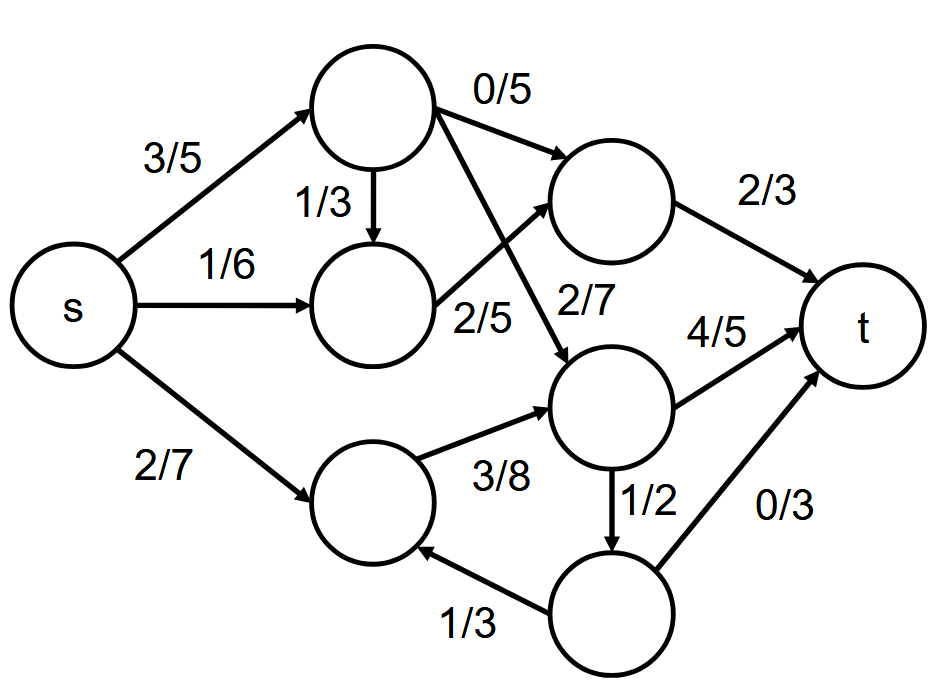
\includegraphics[scale=0.3]{Pics/Flussgraph.png}
    \captionof{figure}{|f| = 6, nicht maximal, da z.B. über obere Kanten noch +1 könnte.}
\end{figure}
\begin{figure}[htp]
    \centering
    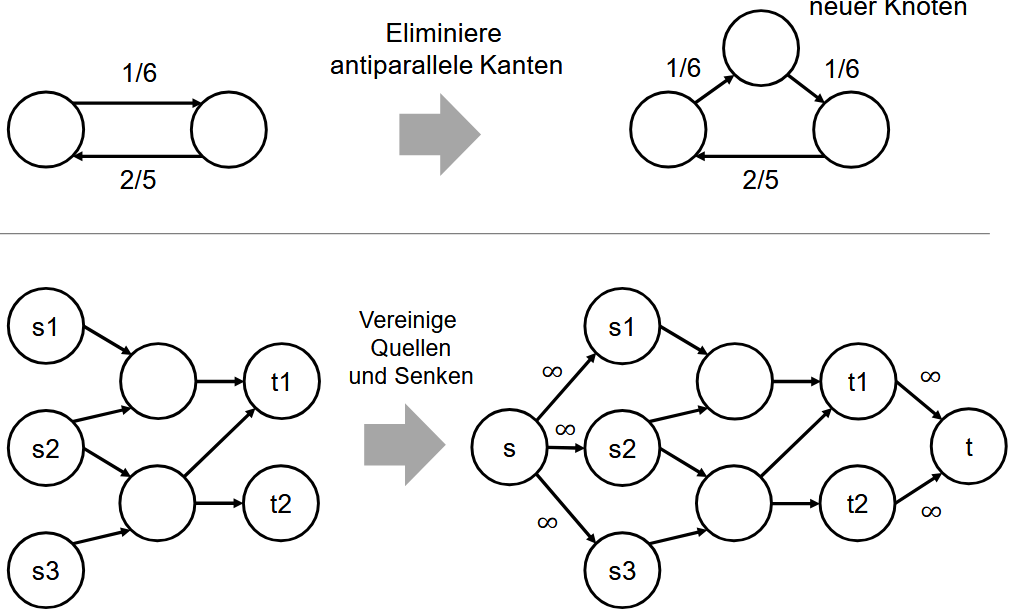
\includegraphics[scale=0.55]{Pics/FlussTransformationen.png}
    \captionof{figure}{Verschiedene Transformationen von Flüssen}
\end{figure}

\subsubsection{Ford-Fulkerson Algorithmus}
Der Ford-Fulkerson Methode zufolge wird im Flussgraphen ein Pfad von s zu t gesucht, der noch erweiterbar bzgl. des Flusses ist. Hierbei wird aber nicht der eigentlich Graph genutzt, sondern der sogenannte Restkapazitätsgraph. Dieser Graph stellt die Restkapazitäten einer Kante aufgeteilt auf Vorwärts- und Rückwärtskante dar. Dabei gilt für die Vorwärtskante $c_f(u,v) = c(u,v) - f(u,v)$ (Wie viel freie Kapazität die Kante hat), wenn (u,v) $\in$ E und die Rückwärtskante $c_f(u,v) = f(v,u)$ (Wie viel Kapazität die Kante schon besetzt), wenn (u,v) $\in$ E. Andernfalls ist $c_f(u,v) = 0$. \\
\begin{figure}[htp]
    \centering
    \includegraphics[scale=0.60]{Pics/FlussRestkapazität.png}
    \captionof{figure}{Formelle Restkapazität}
\end{figure}
\begin{figure}[htp]
    \centering
    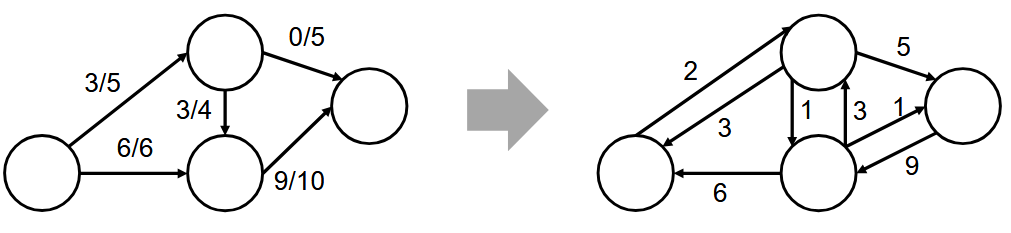
\includegraphics[scale=0.70]{Pics/FlussRKG.png}
    \captionof{figure}{Restkapazitätsgraph}
\end{figure}

Im Restkapazitätsgraph ist es nun also so, dass wenn eine Kante von einem Knoten wegführt, dieser noch Kapazität übrig hat und der Fluss an dieser Kante erhöht werden kann. Demnach muss in diesem Graphen jetzt nur noch ein Pfad von s nach t gefunden werden, dessen Existenz impliziert, dass der maximale Fluss noch nicht erreicht ist. Demnach können auf diesem Pfad die Restkapazitäten angepasst werden. Formell:\\
\textit{Finde Pfad von s zu t in $G_f$ und erhöhe (für Kanten in G) bzw. erniedrige (für nicht-Kanten) um Minimum $c_f(u,v)$ aller Werte auf dem Pfad in G}\\
\begin{algorithm}[H]
    \SetKwFunction{fofuls}{FordFulkerson}
    \tcp{Complexity: $O(|E|\cdot u \cdot |f^*|)$, u = max capacity, $|f^*|$ = max flow}
    \tcp{s start, t target, c capacity function}
    \Fn{\fofuls{G, s, t, c}}{
        \ForEach{e in E}{
            e.flow = 0; \tcp{Initializes all flow values to 0}
        }
        \tcp{goes through every possible path with free capacity}
        \While{path p from s to t exists in $G_f$}{
            $c_{f}$(p) = min\{$c_f$(u,v) : (u,v) \in p\}; \tcp{Minimum of all flow values on the path}
            \tcp{Changes the flow values on the path}
            \ForEach{e in p}{
                \tcp{If edge e in p \rightarrow total flow, else remaining capacity}
                \If{e in E}{
                    e.flow += $c_{f}$(p); \tcp{Add minimal flow to edge}
                }
                \Else{
                    e.flow -= $c_{f}$(p); \tcp{Subtract minimal flow from edge}
                }
            }
        }
    }
\end{algorithm}
\includepdf[pages={187-191}, pagecommand={},nup=2x3, frame=true, scale=0.9]{./VL Folien/06GraphAlgorithms.pdf}

\end{document}